\documentclass[]{article}
\usepackage{graphicx}
\usepackage{indentfirst}
\usepackage{clrscode3e}
\setlength{\parindent}{0pt}
%opening
\title{CLRS Exercise}
\author{Tongda Xu}

\begin{document}

\maketitle
\section{7}
\subsection{7.3}
\subsubsection{a}
This is certain concerning the $Randomized$ procedure, the probability of any index $i$ is chosen from $[0,n-1]$is:\\
$Pr(pivot = i) = \frac{1}{n}$\\
$E(X_{i}) = 1*Pr(pivot = i) + 0*Pr(pivot \neq i) = \frac{1}{n}$

\subsubsection{b}
It is certain that if $ith$ element is chosen as pivot, $Random-Parition$ cost $\Theta(n)$ time, and it will call $QuickSort[1, q-1], QuickSort[q+1, n]$ recursively.\\
Concerning only the first $Parition$, this would be the result:\\
$E(T(n)) = \Sigma_{i=1}^{n}Pr(pivot = i)(T(i-1) + T(n-i) + \Theta(n))\\
 = \Sigma_{i=1}^{n}X_{i}(T(i-1) + T(n-i) + \Theta(n))$
 
\subsubsection{c}
Concerning $X_{i} = \frac{1}{n}\\
E(T(n)) = \Sigma_{i=1}^{n}\frac{1}{n}(T(i-1) + T(n-i) + \Theta(n))\\
= \Sigma_{i=1}^{n}\frac{1}{n}T(i-1) + \Sigma_{i=1}^{n}\frac{1}{n}T(n-i) + \Sigma_{i=1}^{n}\frac{1}{n}\Theta(n)\\
= \frac{2}{n}\Sigma_{i=1}^{n-1}T(i) + \Theta(n)$

\subsubsection{d}
$\Sigma_{k=2}^{n-1}klgk \\
\le lg\frac{n}{2}\Sigma_{k=2}^{\frac{n}{2}}k + lgn\Sigma_{k=\frac{n}{2}}^{n-1}k\\
= lgn\Sigma_{k=2}^{n-1}k - lg2\Sigma_{k=2}^{\frac{n}{2}}k\\
= lgn\frac{(n+1)(n-2)}{2} - \frac{(\frac{n}{2} + 2)(\frac{n}{2}-1)}{2}\\
\le lgn\frac{n^2}{2} - \frac{n^2}{8}$\\
by Calculus, we have:\\
$(\frac{1}{2}x^2lgx - \frac{1}{4}x^2)|_{1}^{n-1} \le E(T(n)) \le (\frac{1}{2}x^2lgx - \frac{1}{4}x^2)|_{2}^{n}$

\subsubsection{e}
Proof of $E(T(n)) = O(nlgn)$:\\
Assume that $\forall k \in [1, n-1], \exists c, E(T(k)) \le cklgk - \Theta(k)$\\
For $k = n, E(T(n)) \le \frac{n}{2}c(lgn\frac{n^2}{2} - \frac{n^2}{4} - \Theta (n^2)) + \Theta(n) \le cnlgn - \Theta(n) $\\
Proof of $E(T(n)) =\Omega(nlgn)$:\\
Assume that $\forall k \in [1, n-1], \exists c, E(T(k)) \ge cklgk + \Theta(k)$\\
For $k = n, E(T(n)) \ge \frac{n}{2}c(lgn\frac{(n-1)^2}{2} - \frac{(n-1)^2}{4} + \Theta(n^2)) + \Theta(n) \ge cnlgn + \Theta(n)$\\
$\rightarrow E(T(n)) = \Theta(nlgn)$

\subsection{7.5}

\subsubsection{a}
From counting Theorem, it could be noticed that:\\
$p_{i} = \frac{(i-1)(n-i)}{C_{n}^{3}} = \frac{6(i-1)(n-i)}{n(n-1)(n-2)}$

\subsubsection{b}
$Pr(i = medium) (normal) = \frac{1}{n}\\
Pr(i = medium) (3part) = \frac{6(\frac{1}{2}n-1)(n-\frac{1}{2}n)}{n(n-1)(n-2)} = \frac{3}{2}\frac{1}{n}\\
Pr(3part) - Pr(normal) = \frac{1}{2}\frac{1}{n}$

\subsubsection{c}
Consider $f_{diff}= {\int }_{\frac{n}{3}}^{\frac{2}{3}n} (\frac{6(i-1)(n-i)}{n(n-1)(n-2)} - \frac{1}{n})di\\
 = \frac{(-2i^3 + 3(n+1)i^2 - 6ni - (n-1)(n-2)i)|_{i = \frac{1}{3}n}^{i = \frac{2}{3}n}}{n(n-1)(n-2)}\\
{lim}_{n\to \infty} f_{diff} = \frac{4}{27}$

\subsubsection{d}
Consider we are so lucky that each partition we choose the median:\\
In the Iteration tree, we have:\\
$ T(n)=\left\{
\begin{array}{lcl}
c       &      & {n = 1}\\
2T(\frac{1}{2}n) + n     &      & {n > 1}\\
\end{array} \right. $\\
The $\Omega(nlgn)$ is kept even in best case.

\section{8}
\subsection{8.1-1}
n-1 times, since we need n elements to formulate
\subsection{8.1-2}
$\Sigma_{1}^{n}lgk < \int_{1}^{n+1}lgkdk = (klgk - k)_{1}^{n} = (nlgn - n) - (0 - 1) = nlgn -n + 1 $
\subsection{8.1-3}

$ \leftrightarrow $ proof at least half of branch is longer than h
\\Consider a decision tree with $n!/2$ elements

$\leftrightarrow$ proof at least half of branch is longer than h
\\Consider a decision tree with $n!/n$ elements

$\leftrightarrow$ proof at least half of branch is longer than h
\\Consider a decision tree with $n!/2^n$ elements, this is not significant enough and could leave only $\Omega (lg\frac{n!}{2^n}) = \Omega(nlgn - n) = \Omega (nlgn)$ elements

\subsection{8.2-4}
Consider a trim version of counting sort, build the $C$ map up and query directly:
\begin{codebox}
	\Procname{$\proc{Counting-sort-trim($A, k$)}$}
	\li $C []$
	\li \For $i \gets 0$ \To $k$
	\li		\Do $C[i] = 0$
	\End
	\li \For $j \gets 1$ \To $A.length$
	\li		\Do $C[A[j]]++$
	\End
	\li \For $m \gets 1$ \To $k$
	\li		\Do $C[m] += C[m-1]$
	\End
	\li \Return $C[m]$
\end{codebox}

\begin{codebox}
	\Procname{$\proc{Direct-Quert($A, k, a, b$)}$}
	\li $C = \proc{Counting-sort-trim($A, k$)}$
	\li \If $a < 1$
	\li \Then \Return $C[b]$
	\li \Else \Return $C[b] - C[a-1]$
\end{codebox}

\subsection{8.3-2}
Heapsort is not stable\\
The scheme would be very similar to counting sort and takes $\Theta(n)$ time

\subsection{8.3-4}
First, with $O(n)$ time: convert n numbers $k_{10}$ into $k_{n}$ which has 3 digits.\\
Second, with $O(d(n+n))$ time ($Lemma8.3$): Radix sort n 3-digit numbers with each digits take up to n possible values.

\begin{codebox}
	\Procname{$\proc{digitsConvert($X$)}$}
	\li $result []$
	\li \For $i \gets 2$ \Downto $0$
	\li		\Do $result[i] = X/n^i$
	\li			$X = X \bmod{n^i}$
	\End
	\li \Return $result$
\end{codebox}

\begin{codebox}
	\Procname{$\proc{sort($A,x$)}$}
	\li $result []$
	\li \For each $S$ in $A$
	\li		\Do $S =\proc{digitsConvert($S$)}$
	\End
	\li \proc{radix-sort($A,x$)}
\end{codebox}

\section{9}

\subsection{9.2-1}
once $p == r$, the function return and recursion end.

\subsection{9.2-2}
It is because $\forall k, X_{k} = \frac{1}{n}$, giving information on which k would not effect observation

\subsection{9.2-3}
\begin{codebox}
	\Procname{$\proc{randomized-select-iter($A,p,r,i$)}$}
	\li \While $1$
	\li	\Do \If $i == k$
	\li  \Then \Return $A[i]$
	\li \Else 
	\li  $q =\proc{random-partition($A,p,r$)}$
	\li 	\If $i < k$
	\li     \Then $r = q-1$
	\li 	\Else $p = q+1, i = i-k$
	\End
	\End
	\End
\end{codebox}

\subsection{9.2-4}
The worst case is reverse side:\\
$pivot = {9,8,7,6,5,4,3,2,1,0}$

\subsection{9.1}
\subsubsection{a}

Sorting: $\proc{Merge-sort($A$)}$ in worst case $O(nlgn)$\\
Query: $\proc{call-by-rank($A,k$)}$ i times in worst case $O(i)$, here we assume manipulating $O(n)$ space cost $O(n)$ time.

\subsubsection{b}

Building: $\proc{build-map-heap($A$)}$ in worst case $O(n)$\\
Query: calling $\proc{Extra-max($A,k$)}$ i times in worst case $O(ilgn)$

\subsubsection{c}

Selecting: $\proc{select($A, i$)}$ in worst case $O(n)$\\
Sorting:  $\proc{Merge-sort($A^{'}$)}$ in worst case $O(ilgi)$

\subsection{9.2}
\subsubsection{a}

$\Sigma_{1}^{k-1} w_{i} = \Sigma_{1}^{k-1} \frac{1}{n} = \frac{k-1}{n} < \frac{1}{2}\\
\Sigma_{k+1}^{n} = \frac{n-k}{n} \le \frac{1}{2}$

\subsubsection{b}

\begin{codebox}
	\Procname{$\proc{weight-median($A$)}$}
	\li w[] = \proc{Sort($A$)}.weight
	\li n = w.length
	\li	\For $i \gets 1$ \To $n$
	\li 	\Do $w[i] = w[i] + w[i-1]$
	\End
	\li \Return \proc{Find($w[], \frac{1}{2}$)}
\end{codebox}

\subsubsection{c}

\begin{codebox}
	\Procname{$\proc{sum($w_{1}, w_{i}, lasti, lastsum$)}$}
	\li \If $i>lasti$
	\li  \Then \Return $lastsum + \proc{ normal-sum( $w_{lasti, i}$ ) }$
	\li  \Else \Return $lastsum - \proc{ normal-sum( $w_{i, lasti} )$ }$ 
	\End
\end{codebox}

\begin{codebox}
	\Procname{$\proc{weight-median-linear($A$)}$}
	\li \While $1$
	\li		\Do \If $sum[w_{1}, w_{i}, lasti, lastsum] < \frac{1}{2}, sum[w_{1}, w_{i+1}, lasti, lastsum] > \frac{1}{2}$
	\li 		\Then \Return $i$
 	\li  	\Else
 	\li 	$lastsum = sum[w_{1}, w_{i}, lasti, lastsum], lasti = i$
 	\li 	\If  $sum[w_{1}, w_{i}] < \frac{1}{2}$
 	\li  		\Then $i = \proc{median($A,i,r$)}$
 	\li 	\Else $i = \proc{median($A,p,i$)}$
 	\End
\end{codebox}

We will experience $logn$ literation, but the load is decreasing logarithmically, so the result is linear. Notice the sum is special here, calculating the difference only.

\subsection{9.4}
\subsubsection{a}
$k \le i $ or $ k \ge j: 0$\\
$i < k < j: \frac{2}{j-i+i}$
\subsubsection{b}
\subsubsection{c}
\subsubsection{d}



\section{11}

\subsection{11.1-2}
Consider $vector<bool> A, a.size() = m$, just store the bool value of $key = m$ exist or not.

\begin{codebox}
	\Procname{$\proc{search($A,key$)}$}
	\li \If $A(key)$
	\li		\Then \Return $key$
	\li  \Else \Return $NIL$
	\End
\end{codebox}

\begin{codebox}
	\Procname{$\proc{insert($A,key$)}$}
	\li $A(key) = 1$
\end{codebox}

\begin{codebox}
	\Procname{$\proc{delete($A,key$)}$}
	\li $A(key) = 0$
\end{codebox}

\subsection{11.2}
\subsubsection{a}

Consider for a ball i fall into a specific bucket $Pr(i) = \frac{1}{n}$\\
Then consider Binomial Distribution, $Pr(k) = C_{n}^{k}Pr(i)^{k}(1-Pr(i))^{n-k}$

\subsubsection{b}

Consider random picking a slot, the probability of that slot is maximum is $Pr_{max} = \frac{1}{n}$, and it contains k elements $Q_{k}$. for conditional probability, we have:\\
$P_{k} = Pr_{i=k|max} = \frac{Pr(i=k \cap max)}{Pr_{max}} \le \frac{Pr(i=k)}{Pr_{max}} = nQ_{k}$

\subsubsection{c}

Proof:\\
$Q_k = (\frac{1}{n})^k(\frac{n-1}{n})^{n-k}C_{n}^{k} \\
= \frac{(n-1)^{n-k}}{n^n} \frac{\Pi_{0}^{k-1}n-k}{k!} \\
\le \frac{n^n}{n^n} \frac{1}{k!}\\
= \frac{e^k}{k^k} \frac{1}{k^{\frac{1}{2}} (1+\Theta(\frac{1}{n}))}\\
\le \frac{e^k}{k^k}$

\subsubsection{d}

Proof for $Q_{k_{0}}$: \\
$Q_{k_{0}} = \frac{e^{(\frac{clgn}{lglgn})}}{(\frac{clgn}{lglgn}) ^ {\frac{clgn}{lglgn}}}\\
= \frac{n^{\frac{clg\frac{e}{c}}{lglgn}}}{\frac{n^c}{n^{\frac{clglglgn}{lglgn}}}} = n^{\frac{clg\frac{e}{c} + clglglgn}{lglgn} - c}$\\
It would not take effort to notice that since ${lim}_{n\to \infty}\frac{clg\frac{e}{c} + clglglgn}{lglgn} =0\\
\forall c > 3+\epsilon, Q_{k_{0}} = O(\frac{1}{n^3}) $\\
And $P_{k} \le nQ_{k} \rightarrow P_{k} = O(\frac{1}{n^2})$

\subsubsection{e}

$E(M) = \Sigma_{M = 1}^{n} M Pr(M) < nPr(M>\frac{clgn}{lglgn}) + \frac{clgn}{lglgn}Pr(M \le \frac{clgn}{lglgn})\\$
A stronger conclusion to note: \\
$E(M) = \Sigma_{M = 1}^{n} M Pr(M) < MPr(M>\frac{clgn}{lglgn}) + \frac{clgn}{lglgn}Pr(M \le \frac{clgn}{lglgn})\\
\le \int_{\frac{clgn}{lglgn}}^{\infty}\frac{1}{n}dn + 1*\frac{clgn}{lglgn} \\
= lg (\frac{clgn}{lglgn}) + \frac{clgn}{lglgn}\\ = O(\frac{clgn}{lglgn})$

\section{15}

\subsection{15.1-1}
$2^n -1 = \Sigma_{j = 0}^{n-1} 2^j $
\subsection{15.1-2}
Do not know how!

\subsection{15.1-3}
\begin{codebox}
	\Procname{$\proc{BOTTOM-UP-CUT-ROD($p, n, c$)}$}
	\li $r[] = c$
	\li  \For $j \gets 1$ \To $n$
	\li    \Do \For $i \gets 1$ \To $j$ 
	\li 		\Do $r[i] = max (p[i] + r[j-i] - c)$
	\End
	\End
	\li \Return $r[n]$
\end{codebox}

\subsection{15.1-4}
\begin{codebox}
	\Procname{$\proc{MEMOIZED-CUT-ROD($p, n, m, s$)}$}
	\li \If $m[n] > -1$ 
	\li 	\Then \Return $m[n]$ \End
	\li  \Else
	\li   \Then \For $i \gets 1$ \To $n$ 
	\li     \Do $m[n] = max (p[i] + r[n-i])$
	\li 	$s[n] = i$ \End
	\li \Return $m[n]$
\end{codebox}

\subsection{15.1-5}
See Code

\subsection{15.2-1}
See Code

\subsection{15.2-2}
See Code

\subsection{15.2-3}

Assume that $\forall k \le n-1, T(k) \ge c2^k$\\
Then $T(n) = \Sigma_{k = 1}^{n-1} T(k)T(n-k) = (n-1)c^22^n > c2^n$\\
So $T(n) = \Omega (n), \omega(n)$

\subsection{15.2-4}
See Figure ~\ref{fig:15.2-4}

\begin{figure}
	\centering
	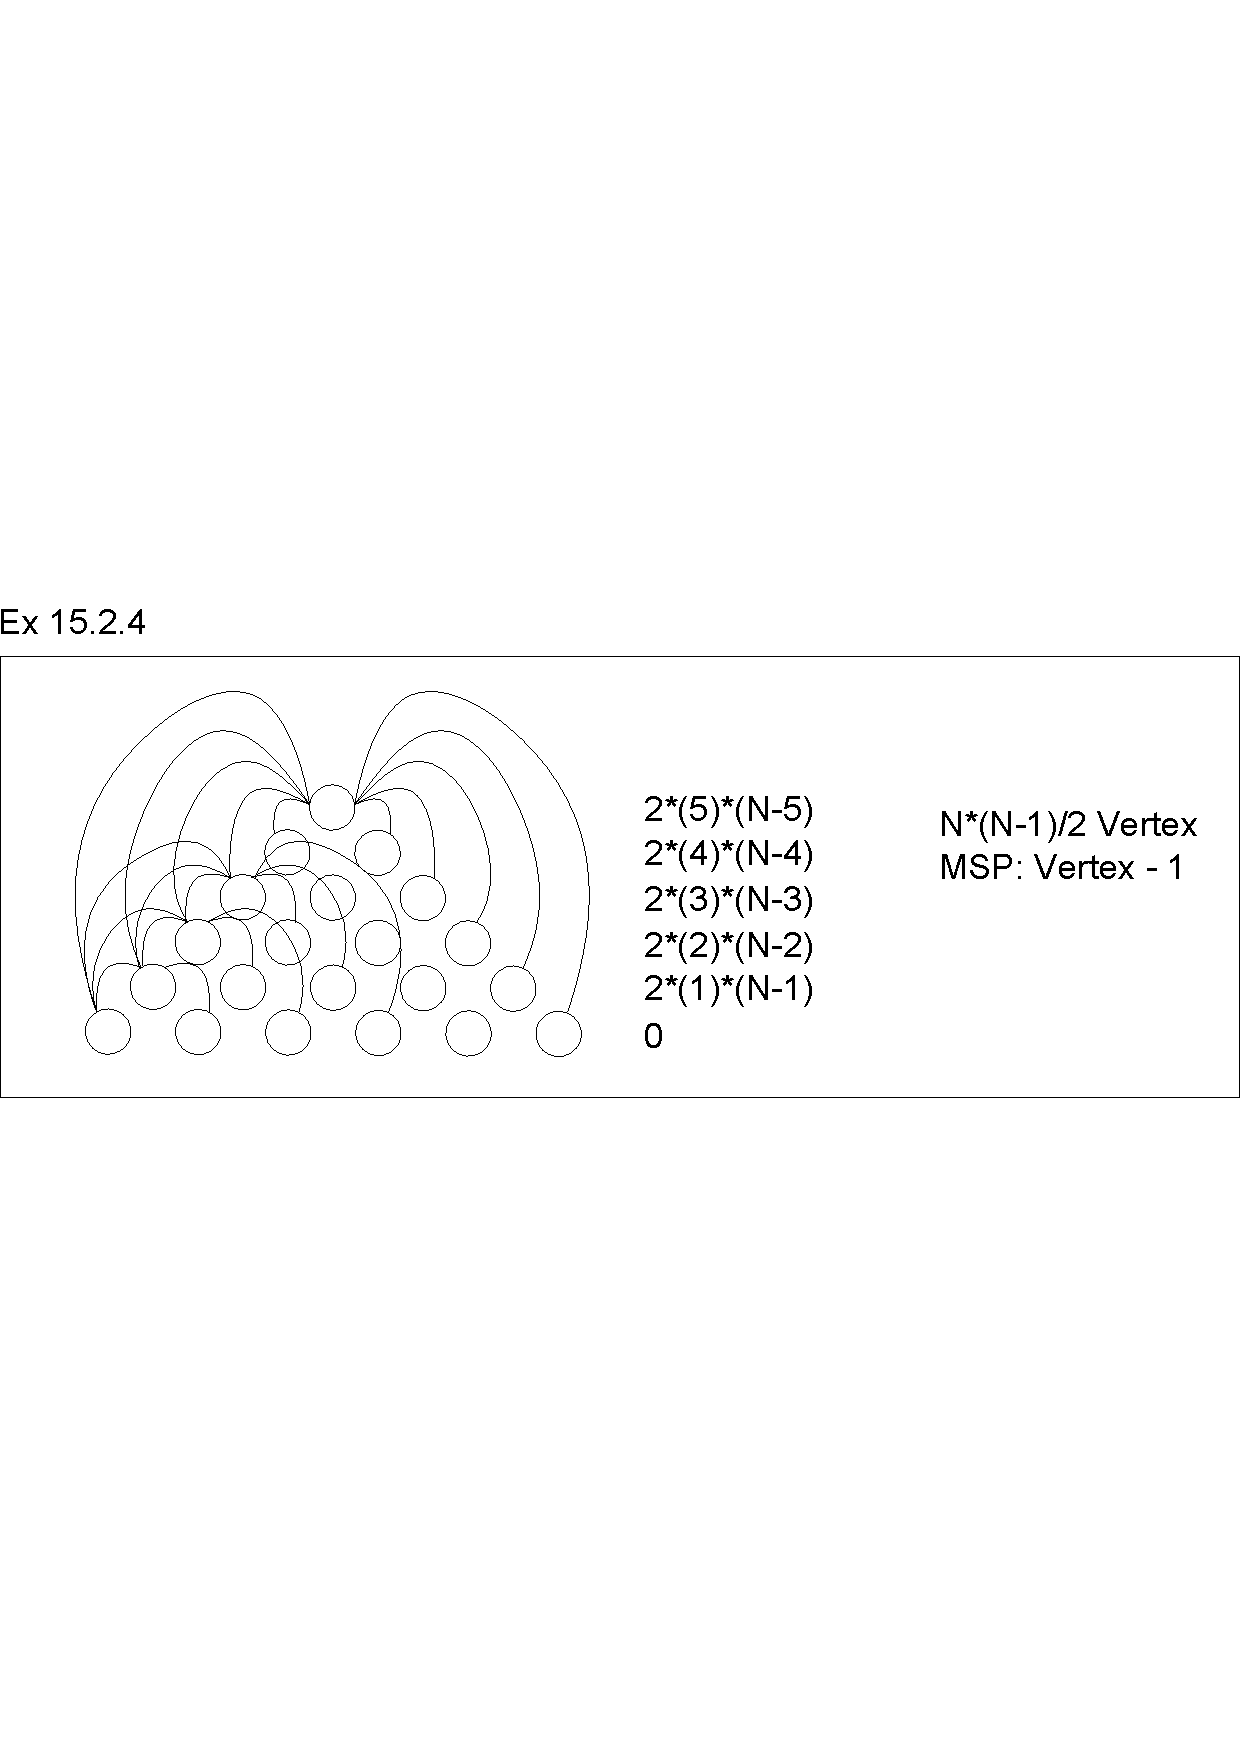
\includegraphics[width=0.8\linewidth]{1524}
	\caption{15.2-4}
	\label{fig:15.2-4}
\end{figure}

\subsection{15.2-5}
For each level $h(i) = i (n-i)$\\
For tree $T(n) = 2\Sigma_{i = 1}^{n-1}i(n-i)
\\ = \frac{3n^3 + 3n^2}{3} - \frac{2n^3 + 3n^2 +n}{3}
\\ = \frac{n^3 - n }{3}$

\subsection{15.2-6}
Assume that $\forall k \le n-1, N(k) = k-1$\\
Then $N(n) = N(n-1) + 1$\\
So $N(n) = n-1$

\subsection{15.3-1}
running through: $T(n) = n*P_{n}^{n} = n*n! > 4^{n}$\\
running recursion: $T(n) = 2\Sigma_{i=1}^{n-1}4^i + n = \frac{8}{3}4^{n-1} + n \le 4^n$\\
running through takes longer

\subsection{15.3-2}
no overlapping subproblem call

\subsection{15.3-3}
Yes

\subsection{15.3-4}
Do not know how!

\subsection{15.4-1}
See code

\subsection{15.4-2}
See code

\subsection{15.4-3}
See code

\subsection{15.5-1}
A Preorder Traverse of BST

\begin{codebox}
	\Procname{$\proc{Pre-Order-Print-Aid($i,j,root$)}$}
	\li \If $root[i,j]-1-i \ge 0$ \Then
	\li k $root[i,root[i,j]-1]$ is the left child of k $root[i,j]$
	\li \proc{Pre-Order-Print-Aid($i,root-1,root[i,root[i,j]-1]$)}
	\li \Else d $i-1$ is the left child of k $root[i,j]$
	\End
	\li \If $j-root[i,j]-1\ge 0$ \Then
	\li k $root[root[i,j]+1, j]$ is the right child of k $root$
	\li \proc{Pre-Order-Print-Aid($root+1,j,root[root[i,j]+1,j]$)}
	\li \Else d $i-1$ is the right child of $root$
	\End
\end{codebox}

\begin{codebox}
	\Procname{$\proc{Pre-Order-Print($root$)}$}
	\li k $root[1,n]$ is the root
	\li \proc{Pre-Order-Print-Aid($1,n,root$)}
\end{codebox}

\subsection{15.5-3}
Asymptotically there would be no change to the running time, just the constant $cn^3$ increase\\
Time spent on $w$ would increase from $\Theta(n^2)$ to $\Theta(n^3)$

\subsection{15.1}

\begin{codebox}
	\Procname{$\proc{LSP($s, t, G$)}$}
	\li $r = G,size()$
	\li $DPs[r] = 0$
	\li $DPr[r] = path(s,t)$
	\li $max = -\infty$
	\li \For $i \gets 1$ \To $r$
	\li		\Do $max (DPs[j] + DPr[r-j] + what)$
	\End
	\li \Return $max$
\end{codebox}

\subsection{15.1}
%subpriblem? vector<string> ()

\subsection{22.1-1}
for both out-degree and in-degree $\Theta (V+E)$ time\\
both take $\Theta (V)$ memory

\subsection{22.1-2}

$1 \rightarrow 2 \rightarrow 3 \rightarrow NIL$\\
$2 \rightarrow 1 \rightarrow 4 \rightarrow 5 \rightarrow NIL$\\
$3 \rightarrow 1 \rightarrow 6 \rightarrow 7 \rightarrow NIL$\\
$4 \rightarrow 2 \rightarrow NIL$\\
$5 \rightarrow 2 \rightarrow NIL$\\
$6 \rightarrow 3 \rightarrow NIL$\\
$7 \rightarrow 3 \rightarrow NIL$

$0-1-1-0-0-0-0$\\
$1-0-0-1-1-0-0$\\
$1-0-0-0-0-1-1$\\
$0-1-0-0-0-0-0$\\
$0-1-0-0-0-0-0$\\
$0-0-1-0-0-0-0$\\
$0-0-1-0-0-0-0$

\subsection{22.1-3}

\begin{codebox}
	\Procname{$\proc{Transpose($Adjlist$)}$}
	\li new $AdjlistPrime$
	\li \For each $node$ in Adjlist
	\li		\Do \For each $subnode$ in $Adjlist(node)$
	\li 		\Do $AdjlistPrime(subnode).insert(node)$
	\li $Adjlist \gets AdjlistPrime$
	\End
\end{codebox}

For adjacent list: just traverse every node and rebuild one\\
$\Theta (E+V)$ for time and space complexity, hard to do it inplace\\

\begin{codebox}
	\Procname{$\proc{Transpose($Adjmatrix$)}$}
	\li \For each $pair(i,j)$ in upper left Adjmatrix
	\li		\Do \proc{Swap($Adjmatrix[i,j], Adjmatrix[j,i]$)}
	\End
\end{codebox}

For adjacent matrix: just transpose the matrix\\
$\Theta (V^2)$ for time and $\Theta(1)$ for space

\subsection{22.1-4}
use an adjacent matrix as aid.

\subsection{22.1-5}

For adjacent list, it is hard. We should regard it as a \proc{Breadth-first-search($G$)} end at $d = 2$:

\begin{codebox}
	
	\Procname{$\proc{square($G$)}$}
	\li \For each $u$ in $G.vertices$
	\li 	\Do $G.reset()$
	\li     $list = \emptyset$
	\li 	$u.adjlist^{'} = \proc{BFS-Aid($G, u, list, 0$)}$
	\End
	\End
\end{codebox}

\begin{codebox}
	
	\Procname{$\proc{BFS-Aid($G, u, list, dist$)}$}
	\li \For each $v$ in $u.adjlist$
	\li 	\Do \If $v.color = white$ and $dist \le 2$ 
	\li			\Then $list.insert(u)$
	\li 		\proc{BFS-Aid($G, v, list, dist+1$)}
	\End=
	\End
	\li \Return $list$
\end{codebox}

This could cost $\Theta(V^2 + VE)$ time and $\Theta(V+E)$ space (if optimized).\\

For adjacent matrix, the square process would be simple. for each index m of matrix row, if matrix[m][n] exist, calculate bool union of matrix[m] and matrix[n]:

\begin{codebox}
	
	\Procname{$\proc{square($G$)}$}
	\li \For each $m$ in $G.adjMatrix$
	\li \Do \For each $n$ $G.adjMatrix[m]$
	\li 	\Do \If $G.adjMatrix[m][n] == 1$
	\li         \Then $G^{'}.adjMatrix[m]$ = \proc{And($G.adjMatrix[m],G.adjMatrix[n]$)}
	\End
	\End
	\End
	\li \Return $G^{'}$
\end{codebox}

The \proc{square($G$)} cost $\Theta(V^3)$ time and $\Theta(V)$ space (if optimize)

\subsection{22.2-3}
line 2 $\rightarrow u.ifgrey = 0$\\
line 5 $\rightarrow s.ifgrey = 1$\\
line 14 $\rightarrow v.ifgrey = 1$

\subsection{22.2-4}
take $\Theta (V^2)$ time and $\Theta (V^2)$ space, since we need to search every column to find adjacent list.\\
line 12 $\rightarrow \textbf{for}: each \quad v \in M[u]$\\
line 13 $\rightarrow \textbf {if}: v == \textbf{true} \quad \textbf{and} \quad v.color == white $

\subsection{22.2-5}

\begin{codebox}
	
	\Procname{$\proc{square($AdjList$)}$}
	\li \For each $u$ in $vertices$
	\li		\Do \For each $v$ in $AdjList(u)$
	\li 		\Do $AdjList(u).append(AdjList(v))$
	\End
	\End
\end{codebox}

For adjacent list, for each vertex u, append the adjacent list of each adjacent vertex v to adjacent list of u.\\
$line 3$ would be execute $\Theta(E)$ times in total, 

\begin{codebox}
	\Procname{$\proc{square($Adjmatrix$)}$}
	\li \For each $pair(i,j)$ in upper left Adjmatrix
	\li		\Do \proc{Swap($Adjmatrix[i,j], Adjmatrix[j,i]$)}
	\End
\end{codebox}

\subsection{Edge traverse of undirected graph}

According to $Theorem 22.10$, all edges are either tree edge or back edge. Modify the \proc{DFS-Visit($G,u$)}, add a \proc{print-path($G,u$)} would do it. Assume a $root = u$ is selected:

\begin{codebox}
	
	\Procname{$\proc{DFS-Visit($G,u$)}$}
	\li $u.color = grey$
	\li $dict[(Vertex,Vertex), edgeType] = \emptyset$
	\li	\For each $v$ in $u.adjList$
	\li \Do \If $v.color == white$
	\li 	\Then $dict(u,v) = treeEdge$
	\li 		  \proc{DFS-Visit($G,v$)}
	\li 	\Else $dict(u,v) = backEgde$
	\End
	\End
	\li \proc{print-path($G,u$)}
	
\end{codebox}

\begin{codebox}
	
	\Procname{$\proc{print-path($G,u$)}$}
	\li \proc{print ($"u"$)}
	\li	\For each $v$ in $u.adjList$
	\li \Do \If $(u,v) == treeedge$
	\li 	\Then \proc{print ($"\rightarrow"$)}
	\li     \proc{print-path($G,v$)}
	\li 	\Else \proc{print ($"\rightarrow v"$)}
	\End
	\End
	
\end{codebox}

line 4,6 cost same level of time as the comparison in line 3, would not change the $\Theta(V+E)$ time complexity of \proc{DFS($G$)}

the print path function as:

This procedure cost $\Theta(V+E)$ as well

\subsection{22.2-6}

Consider the following condition in Figure ~\ref{fig:22.2-6}: \\
$E_{\pi} = <s, u1>, <u1, v1>, <s, u2>, <u2, v2>$\\
In BFS Tree, $\delta (s, v1), \delta (s, v2) $ is either $<s, u1, v1>, <s, u1, v2>$ or $<s, u2, v1>, <s, u2, v2>$

\begin{figure}
	\centering
	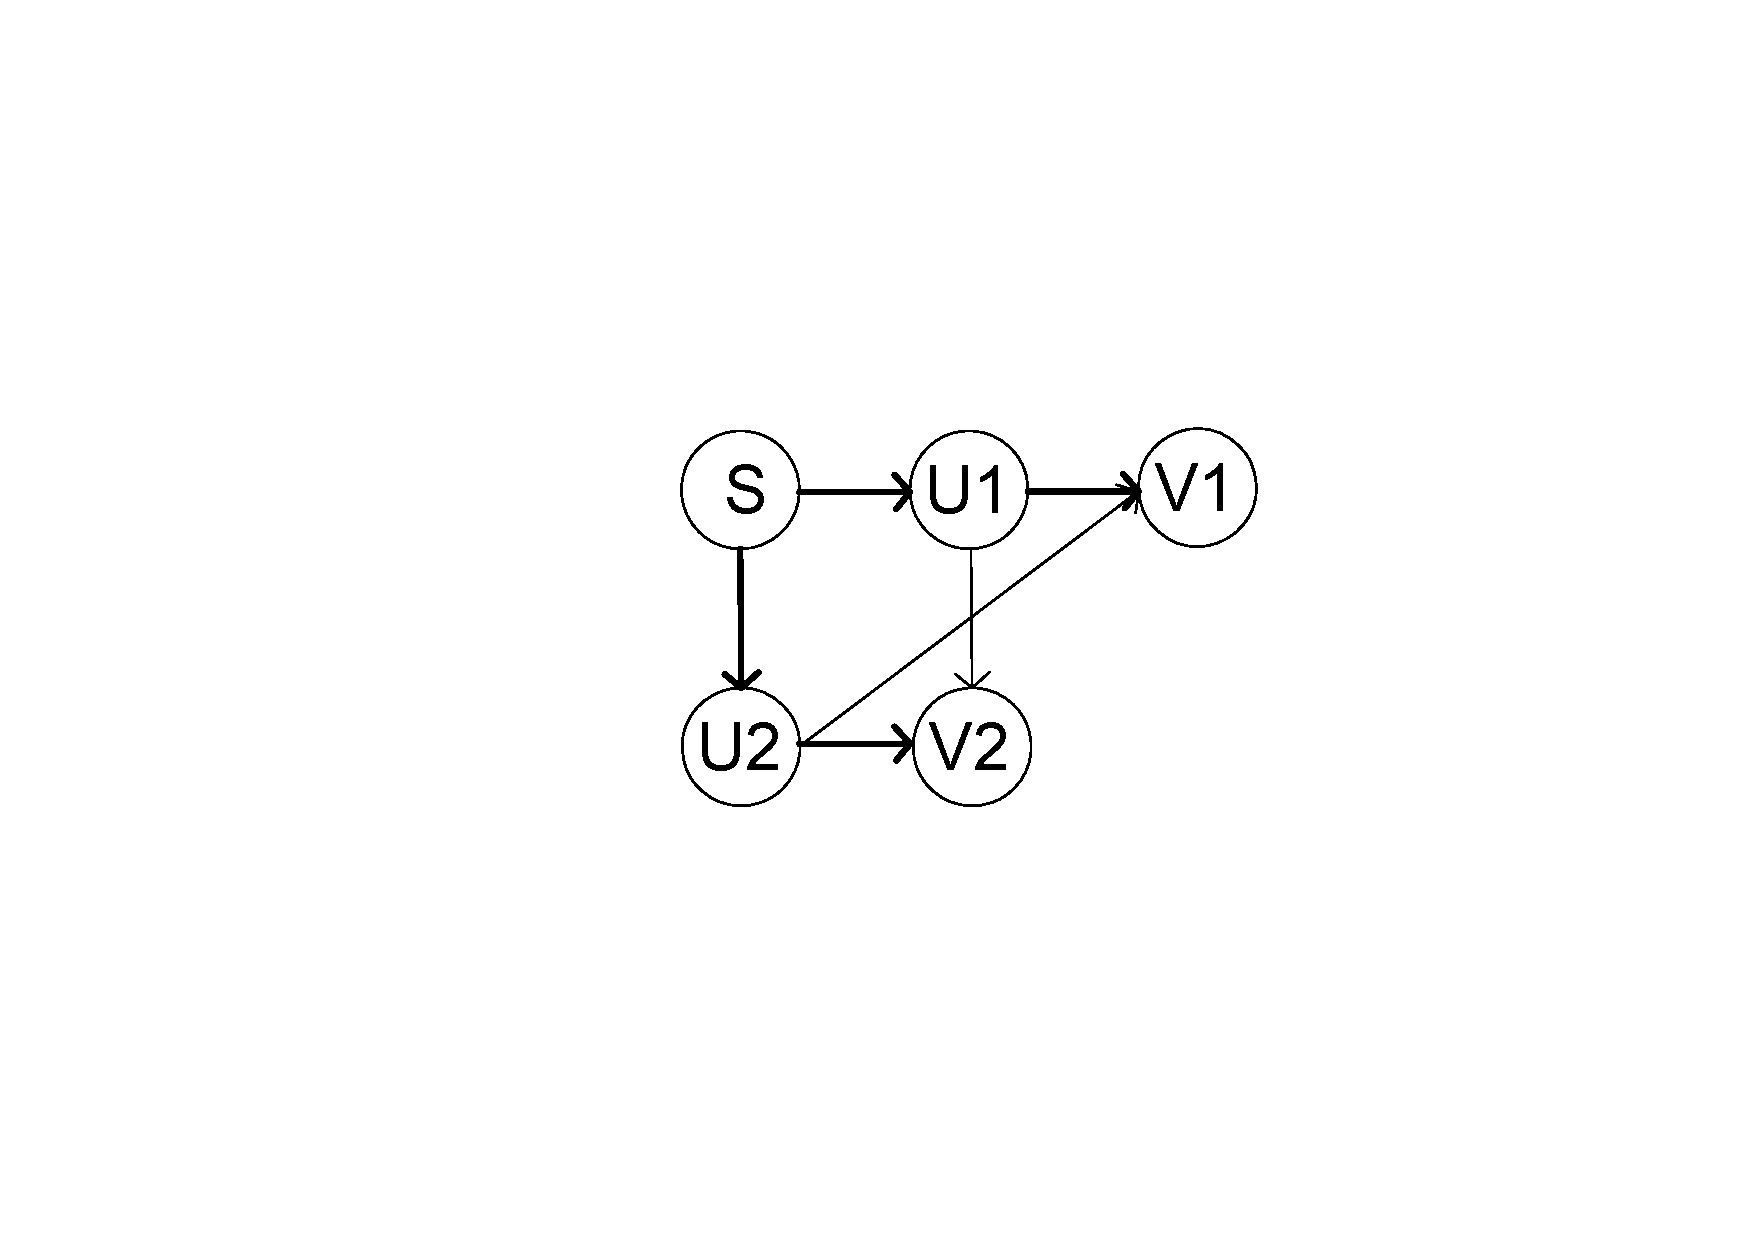
\includegraphics[width=\linewidth]{2226}
	\caption{22.2-6}
	\label{fig:22.2-6}
\end{figure}

\subsection{22-3.12}

Tweak the \proc{DFS-Visit($G,u$)} and \proc{DFS($G$)} would be enough:

\begin{codebox}
	
	\Procname{$\proc{DFS($G$)}$}
	\li	\For each $u$ in $G.V$
	\li \Do $u.color = white$
	\End
	\li $c=1$
	\li	\For each $u$ in $G.V$
	\li \Do \If $u.color = white$
	\li \Then \proc{DFS-Visit($G,u,c$)}
	\li $c$++
	\End
	\End
	
\end{codebox}

\begin{codebox}
	
	\Procname{$\proc{DFS-Visit($G,u,c$)}$}
	\li $u.color = grey$
	\li $u.cc = c$
	\li	\For each $v$ in $u.adjList$
	\li \Do \If $v.color == white$
	\li 	\Then \proc{DFS-Visit($G,v$)}
	\End
	\End
	
\end{codebox}

\proc{DFS($G$)} could be tweaked to do it as well

\subsection{22.4-1}

$ p[27:28] \rightarrow n[21:26] \rightarrow o[22:25] \rightarrow s[23:24] \rightarrow\\
 m[1:20] \rightarrow r[6:19] \rightarrow y[9:18] \rightarrow v[10:17] \rightarrow x[15:16] \rightarrow \\
w[11:14] \rightarrow z[12:13] \rightarrow u[7:8] \rightarrow q[2:5] \rightarrow t[3:4]$

\subsection{22.4-3}
A \proc{DFS($G$)}/\proc{BFS($G$)} returns false when a back edge is found, easy to proof it is $\Theta (V)$

\subsection{22.1}
\subsubsection{a-1}

Suppose $(v,u)$ is a backedge. u is ancestor elder than parent of v. This means $(s,u)$ + forwardEdge is shorter than $(s,v)$ produced by BFS which is $\delta(s,v)$ by \textbf{Theorem 22.5}. Same reason for forward edge.   

\subsubsection{a-2}

By \textbf{Theorem 22.5} $\delta(s,u) = u.d = u.level$ and $\delta(s,v) = v.d =v v.level$, so $v.d = u.d+1$

\subsubsection{a-3}

Same as a-1, if $v.d > u.d + 1$, $\delta(s,v) = (s,u) + cross$ instead of $(s,v)$. if $v.d < u.d$

\subsubsection{b-1}

Same as a-1, the $(s, u) + backEdge$ would be shorter than $(s, v)$

\subsubsection{b-2}

By \textbf{Theorem 22.5} $\delta(s,u) = u.d = u.level$ and $\delta(s,v) = v.d =v v.level$, so $v.d = u.d+1$

\subsubsection{b-3}

Still consider that BFS always generate shortest path. $\delta(s,u) + 1 < (s,v)$ is not allowed

\subsubsection{b-4}

By \textbf{Corollary 22.4} we know that $parenr.d \le child.d$, so for backedge $v.d \le u.d$

\end{document}
